\documentclass{article}
\usepackage{tikz}
\usetikzlibrary{positioning}

\begin{document}

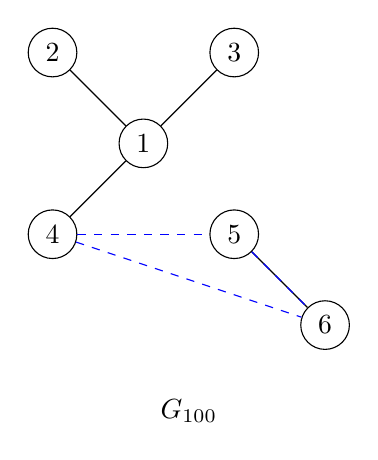
\begin{tikzpicture}[node distance=1cm]
    \node[circle,draw] (1) {1};
    \node[circle,draw,above left=of 1] (2) {2};
    \node[circle,draw,above right=of 1] (3) {3};
    \node[circle,draw,below left=of 1] (4) {4};
    \node[circle,draw,below right=of 1] (5) {5};
    \node[circle,draw,below right=of 5] (6) {6};

    \draw (1) -- (2);
    \draw (1) -- (3);
    \draw (1) -- (4);
    \draw (5) -- (6);

    \draw[dashed,blue] (4) -- (5);
    \draw[dashed,blue] (4) -- (6);
    \draw[dashed,blue] (5) -- (6);

    \node[below=0.5cm] at (current bounding box.south) {$G_{100}$};
\end{tikzpicture}

\end{document}